\documentclass[12pt,a4paper]{report}
\usepackage{svg}
\usepackage{hyperref}
\usepackage{amsmath}
\usepackage{cleveref}
\usepackage{booktabs}
\usepackage{siunitx}
\usepackage{float}
\usepackage{placeins}
\svgpath{{./img}}
\svgsetup{inkscapelatex=false}
\usepackage[spanish]{babel}
\usepackage[utf8]{inputenc}
\usepackage{amsmath, amssymb, graphicx, caption, subcaption, geometry, hyperref}
\geometry{margin=2.5cm}


\usepackage{cleveref}

\crefname{figure}{la figura}{las figuras}
\Crefname{figure}{la Figura}{las Figuras}

\crefname{table}{la tabla}{las tablas}
\Crefname{table}{la Tabla}{las Tablas}

\crefname{section}{sección}{secciones}
\Crefname{section}{Sección}{Secciones}

\crefname{equation}{ecuación}{ecuaciones}
\Crefname{equation}{Ecuación}{Ecuaciones}

\floatplacement{figure}{H}
\floatplacement{table}{H}
\begin{document}

% ---------------------------------------------------------------
% PORTADA
% ---------------------------------------------------------------
\begin{titlepage}
    \centering

    \vfill
\end{titlepage}



% PÁGINA 1 - CARATULA
\begin{center}
UNIVERSIDAD NACIONAL DE TUCUMÁN

FACULTAD DE CIENCIAS EXACTAS Y TECNOLOGÍA

DEPARTAMENTO DE ELECTRICIDAD, ELECTRÓNICA Y COMPUTACIÓN
\vspace*{1cm}


\includegraphics[width=10cm, height=8cm]{./img/logo_unt.png}

\vspace{2cm}



\vspace{2cm}

TRABAJO DE GRADUACIÓN, INFORME FINAL

\vspace{2cm}

Diseño de un ADC SAR de 12 bits @ 40 MSa/s en Tecnología ihp-sg13g2

\vspace{1cm}

Jesus Gerardo Daniel Avila

DNI 41650372

Ing Electrónica 

\vspace{1cm}

Tutores: Miranda Bonomi, Fernando Scandaliaris, Jorge


\vspace{2cm}

Diciembre, 2025

\end{center}

\newpage

% PÁGINA 2 - ANEXO III
\section*{ANEXO III - FICHA DE PRESENTACIÓN DE PROYECTOS FINALES}

\vspace{0.5cm}

\noindent
\textbf{NOMBRE DEL PROYECTO:Diseño de un ADC SAR de 12 bits @ 40 MSa/s en Tecnología ihp-sg13g2}

\vspace{1.5cm}

\noindent
\textbf{APELLIDO(S) Y NOMBRE(S) DEL (DE LOS) ALUMNO(S): Jesus Gerardo Daniel Avila}

\vspace{1.5cm}

\noindent
\textbf{DNI: 41650372}

\vspace{1.5cm}

\noindent
\textbf{OBJETIVOS: Tener un diseño de ejemplo en herramientas Open-Source para la catedra de Diseño de Circuitos Integrados}

\vspace{2.5cm}

\noindent
\textbf{ESPECIFICACIONES: 12 Bits @40MSa/s}

\vspace{2.5cm}

\noindent
\textbf{CONCEPTOS TEÓRICOS PRÁCTICOS INVOLUCRADOS: Diseño VLSI custom}

\vspace{2.5cm}

\noindent
\textbf{DURACIÓN: 7 meses}

\vspace{1.5cm}

\noindent
\textbf{LUGAR DE REALIZACIÓN: Laboratorio Telecomunicaciones (LabTel) - FACET}

\vspace{2cm}

\noindent
\textbf{RESPONSABLE O TUTOR: Miranda Bonomi, Fernando} \hspace{3cm} \\ \\ Firma: \hspace{3cm} Fecha:
\vspace{1.5cm}
\noindent
\textbf{\\ RESPONSABLE O TUTOR: Scandaliaris, Jorge} \hspace{3cm} \\ \\ Firma: \hspace{3cm} Fecha:
\vspace{1.5cm}

\newpage
\chapter*{Dedicatoria}
\thispagestyle{empty}

\vspace*{5cm}

\begin{flushright}
\textit{
A mi Padre, por quien empecé esta carrera\\
A mi Madre, por quien puedo terminarla
}
\end{flushright}

\cleardoublepage
% ---------------------------------------------------------------
% RESUMEN
% ---------------------------------------------------------------
\chapter*{Resumen}
\addcontentsline{toc}{chapter}{Resumen}
Este trabajo presenta el diseño y análisis de un convertidor analógico-digital (ADC) de aproximaciones sucesivas (SAR) de 12 bits operando a 40 MSa/s en tecnología ihp-sg13g2. El diseño implementa un CDAC con arquitectura Inverted Merged Capacitor Switching (IMCS) basada en modo común, un comparador de doble cola tipo Bindra, y lógica SAR síncrona realizada con celdas estándar. Se documentan decisiones de diseño, simulaciones y caracterización del sistema, con énfasis en aspectos didácticos y uso de herramientas de código abierto.

\tableofcontents
\newpage

% ---------------------------------------------------------------
% CAPÍTULO 1: INTRODUCCIÓN
% ---------------------------------------------------------------
% ---------------------------------------------------------------
% CAPÍTULO 1: INTRODUCCIÓN
% ---------------------------------------------------------------
\chapter{Introducción}

\section{Motivación}

Los convertidores analógico-digitales (ADCs) de aproximaciones sucesivas (SAR) son ampliamente utilizados en aplicaciones que requieren eficiencia energética y resoluciones medias-altas. En las últimas décadas, el diseño de SAR ADCs ha experimentado mejoras significativas: se ha conseguido reducir el consumo de energía aproximadamente 7500 veces en un periodo de 15 años~\cite{lowpower_survey}, principalmente gracias al avance hacia nodos tecnológicos más pequeños y al desarrollo de técnicas de conmutación más eficientes.

El presente trabajo documenta el diseño completo de un ADC SAR de 12 bits operando a una velocidad de muestreo mínima de 1~MSa/s, utilizando herramientas de código abierto y la tecnología ihp-sg13g2. El objetivo principal de este trabajo es servir como una primera aproximación al diseño de circuitos integrados, sirviendo como material de referencia para la asignatura de Diseño de Circuitos Integrados de la Facultad de Ciencias Exactas y Tecnología (FACET). 

La elección del SAR ADC como caso de estudio se fundamenta en su complejidad media, que permite ilustrar las diferentes etapas del flujo de diseño analógico sin alcanzar la complejidad de sistemas como PLLs o transceptores completos. Este enfoque didáctico prioriza la documentación exhaustiva del proceso de diseño sobre la optimización extrema del rendimiento.

\section{Estado del Arte}

En un SAR ADC bien optimizado, el retardo~\cite{murmann_sar} (delay) y el consumo de energía~\cite{lowpower_survey} se distribuyen de manera equilibrada entre los tres bloques principales: CDAC, comparador y lógica digital.

\subsection{Evolución de los Comparadores}

El comparador es típicamente implementado con un ancho de banda relativamente pequeño para filtrar el ruido proveniente del CDAC. La arquitectura clásica consiste en un preamplificador seguido de un latch que utiliza realimentación positiva para resolver la decisión. El preamplificador cumple la función de amplificar la señal de entrada y atenuar el offset, ruido y kickback del latch.

Desde la introducción del comparador Strong-ARM, se han propuesto diversas mejoras. Van Elzakker et al.~\cite{vanelzakker_sar} modificaron la topología del latch separando las etapas de preamplificación y regeneración, asegurando que los transistores de entrada del latch comiencen en la región de saturación. Esto resulta en mayor ganancia y reducción del ruido y offset del comparador, mejorando simultáneamente la velocidad de operación.

Más recientemente, Bindra et al.~\cite{bindra_comparator} propusieron un comparador de polarización dinámica (dynamic bias) que alcanza un ruido de entrada de 0.4~mV operando a 1.2~V en tecnología de 65~nm CMOS, mejorando significativamente la eficiencia energética.

\subsection{Arquitecturas de CDAC}

Se han presentado diversas arquitecturas para el CDAC que mejoran sustancialmente la eficiencia energética respecto al esquema convencional~\cite{lowpower_survey}. Entre ellas destacan las arquitecturas basadas en modo común (VCM-based), que mantienen constante el voltaje de modo común durante la conversión, simplificando el diseño del comparador y mejorando la linealidad.

El esquema Inverted Merged Capacitor Switching (IMCS)~\cite{chang_sar_thesis} representa una evolución de estas técnicas, logrando eliminar la sensibilidad a capacitancias parásitas mientras mantiene una alta eficiencia energética (94\% menos consumo que el esquema convencional). Esta arquitectura invierte el proceso de muestreo: durante la fase de muestreo se captura $V_{CM}$ en las placas superiores y la señal de entrada en las placas inferiores, asegurando que las placas superiores comiencen y terminen en el mismo voltaje.

\subsection{Implementaciones Digitales}

Respecto a la lógica de control, se han propuesto tanto diseños full-custom~\cite{murmann_sar} como circuitos auto-sincronizados (self-clocked) para reducir el consumo asociado a la distribución de la señal de reloj. Estos últimos generan los pulsos de control basándose en la detección de la finalización de cada comparación, optimizando la velocidad de conversión.

\section{Resumen del Trabajo}

Este diseño está fuertemente basado en la arquitectura propuesta por Chang~\cite{chang_sar_thesis}, adoptando el esquema de conmutación IMCS y el generador de pulsos auto-sincronizado. La implementación se diferencia en los siguientes aspectos:

\begin{itemize}
    \item \textbf{Herramientas de Código Abierto:} Todo el flujo de diseño se realizó utilizando herramientas libres integradas en el entorno IIC-OSIC-TOOLS: xschem para captura esquemática, ngspice para simulación y klayout para layout. El proyecto completo está disponible en GitHub: \url{https://github.com/gsuckz/SAR_ADC_IHP}.
    
    \item \textbf{Tecnología Abierta:} Se utiliza el PDK ihp-sg13g2, una tecnología de 130~nm completamente abierta y accesible para la comunidad académica.
    
    \item \textbf{Comparador de Polarización Dinámica:} Se implementó el comparador de doble cola propuesto por Bindra et al.~\cite{bindra_comparator}, que incluye un capacitor en la cola del preamplificador para reducir el consumo de potencia.
    
    \item \textbf{Lógica con Celdas Estándar:} A diferencia de implementaciones full-custom, la lógica SAR se realizó con celdas estándar disponibles en el PDK, simplificando el diseño y facilitando la replicabilidad.
    
    \item \textbf{Enfoque Didáctico:} El trabajo prioriza la documentación exhaustiva del proceso de diseño sobre la optimización extrema del rendimiento, sirviendo como material educativo para estudiantes de circuitos integrados.
\end{itemize}

\subsection{Alcance y Limitaciones}

Este trabajo atraviesa las diferentes etapas del diseño de circuitos integrados: desde la captura esquemática y simulación hasta el diseño del layout final, verificando DRC (Design Rule Check) y LVS (Layout vs Schematic). Sin embargo, con el objetivo de mantener el enfoque didáctico y la complejidad manejable, se establecieron las siguientes limitaciones:

\begin{itemize}
    \item No se realizaron simulaciones de mismatch (Monte Carlo) ni análisis de corners de proceso, voltaje y temperatura (PVT).
    \item No se implementaron técnicas avanzadas de optimización de parásitos en el layout.
    \item Las especificaciones mínimas establecidas son 12 bits de resolución y 1~MSa/s de velocidad de muestreo, sin restricciones específicas sobre otras métricas como SNDR, SFDR o consumo de potencia.
\end{itemize}
Debido a que no se realizaron simulaciones de ruido ni de variaciones de proceso (mismatch), la única especificación sobre la que se iteró es el tiempo de conversión, intentando reducirlo lo máximo posible. Se detallan los requeriminetos perseguidos en \cref{tab:specs}

\section{Requerimientos del Sistema}

\begin{table}[H]
\centering
\caption{Requerimientos del ADC SAR}
\label{tab:specs}
\begin{tabular}{lc} % Sin líneas verticales
\toprule
\textbf{Parámetro} & \textbf{Valor} \\
\midrule
Resolución & 12 bits (diferencial) \\
Velocidad de muestreo (mínima) & \SI{1}{MSa/s} \\
Velocidad de muestreo (objetivo) & \SI{40}{MSa/s} \\
Tensión de alimentación ($V_{DD}$) & \SI{1.8}{\volt} \\
Tensión de modo común ($V_{CM}$) & \SI{0.9}{\volt} \\
Tecnología & ihp-sg13g2 (\SI{130}{\nano\meter}) \\
Arquitectura CDAC & IMCS con Split 6+6 \\
LSB & \SI{878}{\micro\volt} \\
Tiempo de Muestreo & \SI{2}{\nano\second} \\
\bottomrule
\end{tabular}
\end{table}


\section{Organizacion del documento}
\begin{itemize}
    \item \textbf{Capítulo 2 - Implementación:} Se describe la implementación práctica de cada bloque del ADC SAR: CDAC con esquema IMCS, Switch de Sample \& Hold, comparador de doble cola, lógica SAR y generador de pulsos.
    
    \item \textbf{Capítulo 3 - Layout:} Se adjuntan fotos del layout implementado y se explica la implementacion del CDAC.
    
    \item \textbf{Capítulo 4 - Conclusiones:} Se resumen los resultados obtenidos, lecciones aprendidas y trabajo futuro.
\end{itemize}

Para fundamentos teóricos sobre arquitecturas SAR y esquemas de conmutación, se remite al lector a las referencias citadas~\cite{lowpower_survey, chang_sar_thesis}.

% ---------------------------------------------------------------
% CAPÍTULO 4: DISEÑO DEL CDAC
% ---------------------------------------------------------------
% ---------------------------------------------------------------
% CAPÍTULO 2: IMPLEMENTACIÓN
% ---------------------------------------------------------------
\chapter{Implementación del SAR ADC}
\begin{figure}[H]
	\centering
	\includesvg[width=\linewidth]{tb_sar_adc}
	\caption{Testbench del SAR ADC}
	\label{toptb}
\end{figure}
Este capítulo describe la implementación práctica de cada bloque del ADC SAR de 12 bits. Se detallan las decisiones de diseño, los testbenches utilizados para verificación y los resultados de simulación obtenidos. La \cref{sar_xsc} muestra la interconexion de los bloques principales del sistema.
\begin{figure}[H]
    \centering
    \includesvg[width=\linewidth]{sar_diagrama_xschem}
    \caption{Diagrama de bloques en Xschem}
    \label{sar_xsc}
\end{figure}
\section{Descripcion del SAR ADC nivel TOP}

Como se muestra en la \cref{toptb} las entradas del circuito son $V_{inp}$, $V_{inn}$ y sample, mientras que sus salidas son el vector D[11:0] y la señal de final de conversion eoc (end of conversion). El funcionaminto básico es el siguiente, mientras la señal sample esta en alto todas las salidas del ADC pasan a 0, eoc va a bajo y el ADC está siguiendo la entrada, cuando sample pasa a bajo, el ADC retiene la entrada y empieza a convertir bit a bit, hasta resolver el ultimo bit, cuando resuelve el ultimo bit, eoc se pone a alto indicando que el resultado esta listo, y el ADC queda esperano una nueva señal de sampleo. El hecho que la señal de sample sea externa está pensado para implementar un time-interleaving usando varios canales como este en paralelo coordinados por sus señales de sampleo individuales. Notar que el tiempo de sampleo (sample en 1) se fijó en 2ns (por elección de diseño) y el timing crítico estará en el flanco de bajada de sample (inicio de conversión) ya que la tension de entrada en  este momento será la que se convierta. Un análisis detallado del sampleo en un tiempo no nulo se puede consultar en \cite{iizuka_systematic}. 

\subsection{Arquitectura Inverted Merged Capacitor Switching (IMCS)}
\begin{figure}[H]
    \centering
    \includesvg[width=\linewidth]{imcs_diagrama}
    \caption{Diagrama simplificado de la arquitectua IMCS, usando split dac y capacitores de grounding}
    \label{cdac_simp}
\end{figure}
La arquitectura IMCS (Inverted Merged Capacitor Switching) es una técnica de conmutación para ADCs SAR que representa una evolución de la arquitectura MCS (Merged Capacitor Switching), propuesta por Chang~\cite{chang_sar_thesis}. Esta arquitectura fue seleccionada para el presente diseño por sus múltiples ventajas en términos de eficiencia energética, robustez y simplicidad de implementación. Se ejemplifica de manera simplifcada la arquitectura implementeada en la \cref{cdac_simp}

\subsubsection{Beneficios de la Arquitectura IMCS}

La arquitectura IMCS ofrece las siguientes ventajas respecto a otras técnicas de conmutación:

\begin{itemize}
    \item \textbf{Inmunidad a Capacitancias Parásitas:} A diferencia de otras técnicas eficientes como la conmutación monotónica o la MCS estándar, la arquitectura IMCS garantiza que el voltaje en la placa superior (top-plate) del DAC comience y termine en el mismo voltaje ($V_{CM}$). Esto hace que la precisión de la conversión sea insensible a las capacitancias parásitas en la placa superior del DAC y elimina la dependencia de la inyección de carga con la señal~\cite{chang_sar_thesis}.
    
    \item \textbf{Alta Eficiencia Energética:} La IMCS consume un 94\% menos de energía en comparación con la implementación de conmutación convencional, igualando la eficiencia energética de la arquitectura MCS estándar.
    
    \item \textbf{Modo Común Constante:} Al igual que la MCS, la IMCS mantiene un voltaje de modo común constante durante el proceso de conversión. Esto simplifica el diseño del comparador y mejora la linealidad del ADC al evitar variaciones en el offset dinámico del comparador.
    
    \item \textbf{Rango de Entrada Rail-to-Rail:} Permite un rango de entrada completo (rail-to-rail), lo que maximiza la relación señal-ruido (SNR).
\end{itemize}

La Tabla~\cref{tab:switching_comparison} resume las características principales de las diferentes arquitecturas de conmutación.

\begin{table}[h]
\centering
\caption{Comparación de arquitecturas de conmutación CDAC}
\label{tab:switching_comparison}
\begin{tabular}{|l|c|c|c|c|}
\hline
\textbf{Característica} & \textbf{Conv.} & \textbf{Monotonic} & \textbf{MCS} & \textbf{IMCS} \\
\hline
Consumo relativo & 100\% & 19\% & 6\% & 6\% \\
Sensibilidad parásitos top-plate & Media & Alta & Alta & Baja \\
$V_{CM}$ constante & No & No & Sí & Sí \\
Rango entrada & Limitado & Limitado & Rail-to-rail & Rail-to-rail \\
Capacitancia total & $2^N C_u$ & $2^{N-1} C_u$ & $2^{N-1} C_u$ & $2^{N-1} C_u$ \\
\hline
\end{tabular}
\end{table}

\subsubsection{Funcionamiento del Esquema IMCS}

El nombre ``Inverted'' (Invertido) proviene de la forma en que se realiza el muestreo en comparación con la MCS estándar. El proceso de conversión se desarrolla en las siguientes fases:

\begin{enumerate}
    \item \textbf{Fase de Muestreo:} En lugar de muestrear la señal de entrada en la placa superior, la arquitectura IMCS muestrea el voltaje de modo común ($V_{CM}$) en las placas superiores del array de capacitores y la señal de entrada diferencial ($V_{IN}$) en las placas inferiores. Para una implementación diferencial, las placas inferiores del array positivo se conectan a $V_{INP}$ y las del array negativo a $V_{INN}$.
    
    \item \textbf{Fase de Inversión:} Una vez completado el muestreo, se desconectan las fuentes de entrada mediante la apertura de los switches controlados por las señales non-overlap. Luego, se conecta el voltaje $V_{CM}$ a las placas inferiores de todo el array. Esto empuja la diferencia de voltaje (proporcional a $-V_{IN}$) hacia las placas superiores, donde se encuentra conectado el comparador. El primer bit (MSB) se determina inmediatamente sin consumir energía del array de capacitores.
    
    \item \textbf{Ciclos de Conversión (Bit Cycling):} Dependiendo de la decisión del comparador, los capacitores correspondientes se conmutan desde $V_{CM}$ hacia la referencia positiva ($V_{DD}$) o negativa ($V_{SS}$). El objetivo del algoritmo es llevar el voltaje de la placa superior de regreso a $V_{CM}$ paso a paso, reduciendo el error en cada ciclo mediante búsqueda binaria. Este proceso se repite para cada uno de los 12 bits de resolución.
\end{enumerate}

% FIGURA: Diagrama esquemático mostrando las tres fases de operación del esquema IMCS: muestreo invertido, inicialización y ciclos de conversión

En resumen, la IMCS combina la eficiencia energética de la MCS con la robustez frente a parásitos de las arquitecturas de muestreo en placa inferior (bottom-plate sampling). Aunque la arquitectura IMCS también permite implementar redundancia con ventanas de tolerancia simétricas, esta característica no fue implementada en el presente diseño, optando por una configuración binaria pura de 12 bits.

La característica distintiva que hace a la IMCS insensible a parásitos es que los voltajes en las placas superiores comienzan en $V_{CM}$ y convergen hacia $V_{CM}$ al final de la conversión, eliminando el efecto de las capacitancias parásitas en la precisión de la conversión.

% ---------------------------------------------------------------
\newpage
\section{DAC Capacitivo (CDAC)}

El CDAC implementa el esquema de conmutación IMCS (Inverted Merged Capacitor Switching) con una arquitectura split-binary de 6 bits MSB + 6 bits LSB sin redundancia, para un total de 12 bits de resolución.
Esta arquitectura incluye por cada capacitor 4 switches (Una Transmission Gate para conectar $V_{in}$, otra para conectar $V_{cm}$, un PMOS para conectar a VDD y uno NMOS para conectar a aVSS) en la bottom plate, y 4 swtiches generales que manejan las Top plates del MSB y LSB del lado positivo como del negativo para el sampleo.
Además se agregaron capacitores de grounding para solucionar prblemas de implementación del capacitor de puente (C bridge, $C_B$) y de overrange en el Sub-DAC\cite{chang_sar_thesis}.

\subsection{Definición del Capacitor Unitario ($C_u$)}

\subsubsection{Criterio de Ruido Térmico}

El tamaño del capacitor unitario se determina principalmente por el compromiso entre ruido térmico ($kT/C$) y área de silicio. Para un ADC de 12 bits, el ruido térmico total debe ser suficientemente pequeño para no degradar el número efectivo de bits (ENOB).



Donde $k$ es la constante de Boltzmann, $T$ la temperatura absoluta, $V_{ref}$ el voltaje de referencia y $N$ la resolución en bits.
Como se índica en la figura, el número efectivo de bits (Efective Number of Bits, ENOB) decrece con la magnitud del ruido térmico. En nuestro caso, buscaremos perder menos de 1 bit de ENOB, por lo que buscaremos un ruido térmico menor a 0,5 LSB.

%TODO: Agregar imagen del ENOB vs LSB


El criterio utilizado establece que la capacitancia total del array debe satisfacer, usamos T=300K:
\begin{equation}
C_{total} > \frac{kT\cdot 2^{N+1}}{V_{ref}^2 }
\end{equation}
\begin{equation}
C_{total} >  85,7fF
\end{equation}

Esto refiere a la capacidad total del CDAC. Para obtener el valor unitario debemos dividirlo en la cantidad de capacitores unitarios "vistos" por el switch de muestreo y retención (sample \& hold, S\&H). Esto se aclara en la sección 2-1-3, en este caso son:

\begin{equation}
C_{total} = C_{MSB} + C_{LSB}  
\end{equation}
\begin{equation}
 C_{MSB}=63C_u  \space , \space  C_{LSB} = 63 C_u + C_x=63C_U + 31_cu  \space , \space 
\end{equation}
\begin{equation}
C_{total} = 63C_u + (63C_u+31C_u) = 157C_U
\end{equation}
Finalmente:
\begin{equation}
C_u >= C_{totalmin}/157
\end{equation}
\begin{equation}
C_u >= 0,54 fF
\end{equation}
%TODO reemplazar n
% TODO: Agregar cálculo numérico específico mostrando C_total mínimo

\subsection{Implementación del Array Split-Binary}
Para 
El array se divide en:
\begin{itemize}
    \item \textbf{MDAC (Main DAC):} 6 bits MSB con capacitores pesados binariamente: $32C_u$, $16C_u$, $8C_u$, $4C_u$, $2C_u$, $1C_u$
    \item \textbf{Capacitor de puente:} $C_B = 2C_u$
    \item \textbf{SDAC (Sub DAC):} 6 bits LSB con capacitores pesados binariamente: $32C_u$, $16C_u$, $8C_u$, $4C_u$, $2C_u$, $1C_u$
    \item \textbf{Capacitor de grounding:} $C_X = 31C_u$ en paralelo con el SDAC
\end{itemize}

\subsubsection{Selección del capacitor unitario $C_u$}

Se utilizaron capacitores MIM (Metal-Insulator-Metal) del PDK ihp-sg13g2 por simplicidad en el diseño del layout.
\begin{itemize}
    \item En la documentacion no se indica el coeficiente de matching
    \item Bajo coeficiente de tensión y temperatura
    \item Estructura planar que facilita el layout centroide común (common-centroid)
    \item Se partió del tamaño mínimo permitido por el proceso para un mimcap, $W_c=L_c=1.15\mu m \space \space \textit{con} \space\space C=2.16fF$
    \item A través de iteraciones sobre la simulación TOP se encontró que era necesario un capacitor mucho más grande para lograr una conversión correcta. Algunos efectos que son mitigados por aumentar $C_u$ son: Inyección de carga, corrientes de fuga, ruido por Kickback del comparador. Mediante simulaciones iterativas a nivel de sistema, se observó que el valor mínimo teórico era insuficiente debido a efectos de segundo orden como la inyección de carga y el kickback noise del comparador. Se seleccionó finalmente un capacitor unitario $W_c=L_c=3\mu m \space \space con \space \space C=13.9fF$ , lo cual provee un margen de robustez adicional.
    
\end{itemize}

El capacitor unitario implementado tiene un valor de \textbf{$C_u = 15$ fF} con dimensiones de 3 µm × 3 µm.

% FIGURA: Vista en corte y layout del capacitor MIM unitario del PDK ihp-sg13g2




% FIGURA: Esquemático completo del CDAC diferencial con nomenclatura de cada capacitor



\subsection{Cálculo de Capacitores de Atenuación ($C_B$) y Grounding ($C_X$)}

\subsubsection{Problema del Capacitor Fraccional}

En arquitecturas split-binary, el capacitor de puente ($C_B$) que conecta los segmentos MSB y LSB tradicionalmente tiene un valor fraccional:
\begin{equation}
C_B = \frac{2^L - 1}{2^L} C_u
\end{equation}

Para $L = 6$ bits en el segmento LSB, esto resulta en $C_B = 63/64 \cdot C_u$, un valor no entero que dificulta el matching en el layout.

\subsubsection{Problema de los rieles del Sub-DAC}
Los rieles del sub-dac pueden salir de los rieles de alimentación, como se explica en ~\cite{chang_sar_thesis}. Esto puede producir que las junturas de drenador de los switches se polaricen en directa, por ejemplo, si el drenador de un pmos (con sustrato a vdd) se va arriba de VDD por encima de la tensión de umbral de esta juntura $V_{th_p}=0.48V$ posiblemente dañanado el chip.

\subsubsection{Metodología de Cálculo}

Para resolver ambos problemas, se implementó la arquitectura propuesta por Chang~\cite{chang_sar_thesis}, que introduce un capacitor de grounding ($C_X$) permitiendo que $C_{BX}$ sea un valor entero de unidades $C_u$.

Se adjunta un archivo de  Maxima (disponible en el repositorio GitHub: \url{https://github.com/gsuckz/SAR_ADC_IHP}) que calcula el valor de $C_X$ (como multiplo de $C_u$).


%Completar descripcion del algoritmo 

% FIGURA: Diagrama del CDAC split-binary mostrando MDAC, SDAC, C_B y C_X

\subsubsection{Valores Finales}

Los valores calculados son:
\begin{itemize}
    \item $C_B = 2 \cdot C_u = 27.8 fF$
    \item $C_X = 31 \cdot C_u = 430.9 fF$
\end{itemize}

Estos valores permiten:
\begin{itemize}
    \item Fabricación precisa con matching controlado (valores enteros)
    \item Prevención de over-range en el nodo LSB durante conmutaciones
\end{itemize}

Sin embargo, los pasos del LSB estaban atenuados, por lo que se iteró sobre el $W_B$ al aumnetar el valor de $C_B$ se puede disminuir la atenuaciòn e incluso hacer los pasos mas grandes de lo necesario, se encontro que el valor $W_B=3.23\mu m $ entrega los pasos correctos. Se procedió como sigue:
\begin{itemize}
    \item Se calcula la atenución A del paso como:\\
    $ A = \frac{V_{PasoReal}}{V_{PasoIdeal}}$
    \item Se divide $W_B$ por la atenuación obtenida, tal que:\\
    $W_{B \space nuevo} = \frac{W_B}{A} $
    \item Volver a calcular A
    \item Repetir hasta encontrar un valor aceptable ($A\approx1$)
\end{itemize}

\subsection{Logica de las señales de control de la Bottom Plate de cada celda}

Cada capacitor unitario del array implementa el esquema IMCS mediante la siguiente lógica de switches:

\begin{figure}[H]
    \centering
    \includesvg[width=\linewidth]{dac_unit_cell}
    \caption{Esquema de la lógica de la celda unitaria del DAC, notar que se indican los dispositivos escalados por unidad de capacitor. La cadena de buffers solo es ilustrativa.} 
    \label{botcdac}
\end{figure}

\begin{figure}[H]
    \centering
    \includesvg[width=\linewidth]{dac_unit_cell_n}
    \caption{Celda con bit negado. La cadena de buffers solo es ilustrativa.}
    \label{botcdacn}
\end{figure}
\subsubsection{Switches de Placa Inferior (Bottom Plate)}
La lógica para activar los swtiches segun las señales B[n] y D[n] se detallan en \cref{botcdac} y \cref{botcdacn}
\begin{itemize}
    \item \textbf{Conexión a entradas ($V_{INP}$, $V_{INN}$):} Transmission gates con dummies para minimizar charge injection durante el muestreo
    \item \textbf{Conexión a modo común ($V_{CM}$):} Transmission gates sin dummies (switching durante conversión)
    \item \textbf{Conexión a $V_{DD}$ (referencia):} Transistor PMOS individual
    \item \textbf{Conexión a $V_{SS}$ (tierra):} Transistor NMOS individual
\end{itemize}

Los transistores PMOS y NMOS tienen el mismo tamaño que los transistores que componen los transmission gates para mantener simetría en las impedancias de conmutación.


\subsection{Generador de Señales Non-Overlap}
\begin{figure}[H]
    \centering
    \includesvg[width=\linewidth]{nol_diagrama}
    \caption{Diagrama del generador de señales de sampleo sin superposición}
    \label{noldiag}
\end{figure}



\subsubsection{Funcionamiento}

El generador de pulsos de \cref{noldiag} produce dos señales para el sampleo ($Sample_A$ y $Sample_B$), la primera es la que conecta las  Top Plates a $V_{cm}$, mientras que la segunda conecta las Bottom Plates a $V_{in}$. Funciona de la siguiente manera:
\begin{itemize}
    \item $Sample_A$ y $Sample_B$ cierran sus switches cargando los capacitores del CDAC
    \item $Sample_A$ Abre, dejando flotantes las TOP Plates
    \item $Sample_B$ Abre, desconectando las Bottom Plates de $V_{in}$, cuando esto sucede, la lógica correspondiente a esa celda del CDAC, conecta la Bottom plate a $V_{cm}$ de acuerdo a ala arquitectua IMCS. Permanecerá conectada, hasta que se decida el bit correspondiente a la celda.
\end{itemize}

Este procedimiento evita que los capacitores pierdan carga si se conectaran ambas placas al mismo potencial $V_{cm}$. Para asegurar el NOL se realizó esta implementación a lazo cerrado, por lo que el tiempo muerto incluye todos los delays de los buffers. Las señales se muestran en \cref{nolsalidas}, se indica el delay en \cref{nolsalidas2}


\begin{figure}[H]
    \centering
    \includesvg[width=\linewidth]{nol_salidas_editado}
    \caption{Salidas del NOL, se resalta el tiempo muestro donde ambas señales abren los switches}
        \label{nolsalidas}
\end{figure}

\begin{figure}[H]
    \centering
    \includesvg[width=\linewidth]{nol_formas_de_onda_editado}
    \caption{Señales generadas por el NOL, se señala el alto delay generado por la operacion a lazo cerrado}
    \label{nolsalidas2}
\end{figure}
\subsection{Top Plate Sample switch}

Se implementaron 4 compuertas de transmisión, 2 para los nodos de las TOP plates MSB y LSB de cada parte del DAC

\subsection{Requerimiento de Settling}

\subsubsection{Presupuesto de Tiempo}

Para una velocidad de muestreo objetivo de 40 MSa/s (período de 25 ns), adoptamos un tiempo de muestreo (Tiempo de sampling) $T_s=2ns$, restándonos 23ns para realizar la conversión. Por lo que nuestra señal se debe estabilizar en menos de ese tiempo (tiempo de settiling en la respuesta al escalón). Además buscaremos que el ancho de banda 3dB (BW) del S\&H sea al menos 20 veces mayor a la frecuencia de Nyquist de este ADC, en este caso buscamos un $BW = 400MHz$. En \cref{respuestaac} se muestra el resultado al samplear una señal con $f_1=4*f_{nyquist}$

Usaremos la regla practica de \cite{bwsah}:
$$BW = \frac{0.35}{T_r}$$
$$T_r = \frac{0.35}{BW}$$
$$T_r = \frac{0.35s}{400*10^6}=875ps$$



\subsection{Dimensionamiento del Transmission Gate (sample) }
Se realizó un test bench con el objetivo de alcanzar una respuesta al escalon con un tiempo de settling menor a $875ps $. Para el mismo se colocó una compuerta de transmission  con dummies, el capacitor y una compuerta de transmission sin dummies, como decision de diseño, las dimensiones de $W_n$ y $W_p$ serán las mismas para todas las compuertas.  \\

\begin{figure}[H]
    \centering
    \includesvg[width=\linewidth]{tb_top_tran_step}
    \caption{Testbench usado para probar el $T_r$ del S\&H}
\end{figure}


Se Realizaron las siguientes pruebas:
\begin{itemize}
    \item Se busco un tiempo de settling menor a 875ps para test bench de la figura
    \item Se comprobó el efecto de agregar dummies para mitigar la inyeccion de carga, además se probó la dependencia de este metodo respecto a tiempo de bajada de la señal de sample. \cref{cvssdum} \cref{cvssdumzoom}
    \item Se comprobó que si ponemos n compuertas en paralelo manejan n capacitores igual, el tiempo de rise se mantiene. \cref{risetopa}
    \item Se probó la respuesta al escalon en la señal de sample (tiempo que tarda el switch en cerrar) y luego se probó la respuesta a los 2 escalones en simultaneo. \cref{escalones}
\end{itemize}
\begin{figure}[H]
    \centering
    \includesvg[width=\linewidth]{rise_top}
    \caption{Respuesta al escalón (subida)}
        \label{risetop}
\end{figure}

\begin{figure}[H]
    \centering
    \includesvg[width=\linewidth]{rise_topa}
    \caption{Respuesta al escalón de varios en paralelo (v\_top1a) se observa que se superpone con la respuesta de 1 solo conjunto (v\_top1)}
        \label{risetopa}
\end{figure}


\begin{figure}[H]
    \centering
    \includesvg[width=\linewidth]{delays_sah}
    \caption{Respuesta del circuito con escalon en: entrada (v\_top1), señal de sampleo(v\_top\_sample) y en ambos (v\_top)}
        \label{escalones}
\end{figure}

\begin{figure}[H]
    \centering
    \includesvg[width=\linewidth]{respuesta_c}
    \caption{Ejemplo de sampleo de una señalde 80MHz (4veces la frecuencia de Nyquist)}
    \label{respuestaac}
\end{figure}

\begin{table}[h]
\centering
\caption{Dimensiones del Transmission Gate}
    \label{tgmedidas}
\begin{tabular}{|l|c|}
\hline
\textbf{Parámetro} & \textbf{Valor} \\
\hline
$W_n$ / $L_n$ & 1.0 µm / 0.13 µm \\
$W_p$ / $L_p$ & 2.0 µm / 0.13 µm \\
Tiempo de settling objetivo & $<875$ ps \\
\hline
\end{tabular}
\end{table}


\subsection{Compensación de Inyección de Carga con Dummies}
\begin{figure}[H]
    \centering
    \includesvg[width=\linewidth]{tg_diagrama_dummies}
    \caption{Transmission gate implmentada usando dummies para mitigar la inyección de carga}
   \label{tgdiagdum}
\end{figure}
\subsubsection{Problema de Charge Injection}

Cuando los transmission gates se abren, la carga almacenada en el canal de conducción se inyecta parcialmente en el capacitor de muestreo, introduciendo un error dependiente de la señal.

\subsubsection{Implementación de Dummies}

Se implementaron transistores dummy conectados con compuerta controlada por la señal complementaria. Partiedo de que la capacidad de canal se descarga a través de Source y Drain por igual, por lo que un transistor igual, con la mitad del area (en este caso w) absorberá la mitad de la carga que iría de otra forma al capacitor. Las  \cref{cvssdum} y \cref{cvssdumzoom} y  muestran que para que esta compensacion sea efectiva necesitamos un tiempo de bajada corto. 
\begin{equation}
W_{dummy} = 0.5 \times W_{active}
\end{equation}

\begin{figure}[H]
    \centering
    \includesvg[width=\linewidth]{sample_rapido_vs_lento_dummies}
    \caption{Dependencia de la compensación con dummies del falltime de la señal de sample}
        \label{cvssdum}
\end{figure}
\begin{figure}[H]
    \centering
    \includesvg[width=\linewidth]{sample_rapido_vs_lento_dummies_zoom}
    \caption{Dependencia de la compensación con dummies del falltime de la señal de sample (zoom)}
        \label{cvssdumzoom}
\end{figure}





\subsection{Testbench del CDAC}

\subsubsection{Objetivo del Test}

El testbench valida:
\begin{enumerate}
    \item Tiempo de settling de cada paso de conversión
    \item Valores correctos de los saltos de tensión (verificación de atenuación)
    \item Funcionamiento correcto de ambos sub-arrays (MDAC y SDAC)
    \item Comportamiento del esquema de conmutación IMCS
\end{enumerate}

\subsubsection{Configuración del Test}

% FIGURA: Diagrama del testbench del CDAC mostrando generadores de señales, CDAC bajo test y puntos de medición

El testbench implementa:
\begin{itemize}
    \item Generadores de voltaje para $V_{INP}$, $V_{INN}$, $V_{CM}$, $V_{DD}$
    \item Bloque lógica SAR para obtener el delay total desde la decisión del comparador
    \item Medición diferencial en las placas superiores del CDAC
    \item Análisis transitorio para observar settling
\end{itemize}

\subsubsection{Resultados}

\begin{table}[H]
\centering
\caption{Valores de salto de tensión en el CDAC - Verificación del esquema IMCS}
\label{tab:cdac_voltage_steps}
\begin{tabular}{ccccc}
\toprule
\textbf{Salto} & \textbf{Segmento} & \textbf{$V_{\text{dacP}}$ (mV)} & \textbf{$V_{\text{dacN}}$ (mV)} & \textbf{$V_{\text{dac,diff}}$ (mV)} \\
\midrule
0 & Main DAC & $401.017$ & $401.014$ & $802.439$ \\
1 & Main DAC & $200.648$ & $200.649$ & $401.297$ \\
2 & Main DAC & $100.351$ & $100.285$ & $200.636$ \\
3 & Main DAC & $50.188$ & $50.142$ & $100.331$ \\
4 & Main DAC & $25.097$ & $25.064$ & $50.0161$ \\
5 & Main DAC & $12.549$ & $12.53$ & $25.079$ \\
\midrule
6  & Sub DAC & $6.359$ & $6.368$ & $12.72$ \\
7 & Sub DAC & $3.185$ & $3.167$ & $6.352$ \\
8 & Sub DAC & $1.592$ & $1.582$ & $3.174$ \\
9 & Sub DAC & $0.79$ & $0.79$ & $1.59$ \\
10 & Sub DAC & $0.397$ & $0.397$ & $0.794$ \\

\end{tabular}
\end{table}

Se implementaron las compouertas con las medidas detallas en \cref{tgmedidas}. Se puede observar en los cuadros 2.3 y 2.4 que los pasos decrecen exponencialmnte, y que estan atenuados respecto a los esperado por un factor de $0.89$. Se observa además que la operación en amvos CDAC (lado p y lado n) son prácticamente simétricos.

% FIGURA: Formas de onda del testbench mostrando settling en cada paso de conversión
% FIGURA: Gráfico de los saltos de tensión vs bit position mostrando la atenuación correcta

\begin{table}[H]
\centering
\caption{Parámetros del CDAC}
\begin{tabular}{|l|c|}
\hline
\textbf{Parámetro} & \textbf{Valor} \\
\hline
Capacitor unitario ($C_u$) & 13.9 fF \\
Tipo de capacitor & MIM 3µm × 3µm \\
Capacitor de puente ($C_B$) & $2 C_u$ = 27.8 fF \\
Capacitor de grounding ($C_X$) & $31 C_u$ = 430 fF \\
Capacitancia total MDAC & $63 C_u$ = 945 fF \\
Capacitancia total SDAC + $C_X$ & $94 C_u$ = 1.3 pF \\
Tiempo de settling promedio (por paso) & $387$ ps \\
Tiempo de settling Maximo (por paso) & $527$ ps \\
\hline
\end{tabular}
\end{table}

% ---------------------------------------------------------------

\newpage

\section{Comparador de Doble Cola}

Se implementó el comparador de doble cola (double-tail) propuesto por Bindra et al.~\cite{bindra_comparator}, que separa las etapas de preamplificación y regeneración para optimizar velocidad y consumo.


El comparador de doble cola (Fig. 2.2) Se compone de 2 etapas, un preamplificador que aporta ganancia a la vez que aislación hacia la etapa anterior (CDAC) y una segunda etapa con un latch regenerativo para realizar la comparación. 


El funcionamiento básico se describe así: cuando di\_clk está en 0, el preamp carga los nodos vcpp y vcpn a VDD. Mientras que el latch descarga sus nodos de salida hacia VSS. Este tiempo se llama tiempo de reset.
Cuando di\_clk está en 1, el preamp empieza a descargar los nodos vcpp y vcpn a través del capacitor de cola. Esto genera una una tensión diferencial en la entrada del latch regenerativo, que determina cual será el estado final de los nodos de salida. De esta manera voutp se va alto si vinp es mayor que vinn y viceversa. Este tiempo de llama tiempo de comparacion.

\subsection{Presupuesto de Tiempos}
Durante el proceso de conversión, se van generando 1 a 1 los bits del código de salida, el tiempo que tarda en decidirse cada bit se denomina tiempo de bit. El tiempo de conversión, será entonces N veces el tiempo de bit, siendo N el número de bits del código.

\subsubsection{Ciclo de Conversión}

Cuando la señal pulse esta en bajo, el comparador realiza la decisión, mientras que durante el tiempo alto la lógica genera el bit de acuerdo a la comparación y de acuerdo a esto el CDAC ajusta su salida. 

En este caso, el tiempo bajo será variable, ya que por la naturaleza del comparador las entradas diferenciales mas pequeñas tomarán mas tiempo en resolverse. En cambio el tiempo alto será fijo debido al generador de pulsos, este tiempo está ajustado de manera de asegurar el settling del DAC antes del flanco de bajada. 
Llamaremos tiempo de settling del CDAC $(T_{settlingCDAC} )$ al tiempo desde que clk sube al 50\% de VDD hasta que las salidas del CDAC alcanzan el 90\% de su valor final. 

Llamaremos tiempo de decision $(T_{decision})$ al tiempo desde que clk baja al 50\% de VDD hasta que el latch sale de metaestaibilidad.

\begin{itemize}
    \item Fase de reset (tiempo alto): Reset del comparador y settling del CDAC
    \item Fase de compacion (tiempo bajo)
\end{itemize}

El presupuesto de tiempos se diseñó considerando:
\begin{equation}
T_{bit} = T_{reset} + T_{comp} > T_{settling\_CDAC} + T_{decision}
\end{equation}

El generador de pulsos asegura esto a través de:
Un tiempo de reset del doble del tiempo estimado de Settling y un tiempo de comparación que termina cuando alguna de las salidas del comparador va a alto, en este tiempo se incluyen entonces el retardo de los buffers y el retardo propio del generador de pulsos.
% FIGURA: Diagrama de timing mostrando las fases de reset y evaluación en un ciclo de bit

\subsection{Arquitectura del Comparador}

El comparador se basa en el diseño de polarización dinámica propuesto por Bindra~\cite{bindra_comparator} indicado en \cref{preampdiag} y \cref{latchdiag}, modificando la arquitectura de Elzakker\cite{vanelzakker_sar} para reducir consumo mediante un capacitor en la cola del preamplificador. Los tamaños se indican en \cref{tab:comparator_detailed_sizing}

Se incluye un generador de pulsos que detecta cuando se realizó la comparación, y genera un tiempo de reset fijo para esperar el settling del DAC. El diagrama del mimsmo se indica en \cref{pgendiag}. En el mismo se incluye un buffer Schmitt Trigger implementado como se indica en \cref{pgenst}.

El funcionamineto se ilustra en \cref{salidascomp} y se muestra su tiempo de reset en \cref{compres}.

\begin{figure}[H]
    \centering
    \includesvg[width=\linewidth]{DT_comparator}
    \caption{Diagrama de Bloques del comparador usado}
        \label{compbloques}
\end{figure}

\begin{figure}[H]
    \centering
    \includesvg[width=\linewidth]{bindra_preamp_diagrama}
    \caption{Preamplificador con Capacitor de Cola}
        \label{preampdiag}
\end{figure}

\begin{figure}[H]
    \centering
    \includesvg[width=\linewidth]{latch_diagrama}
    \caption{Latch del comparador Doble Cola}
        \label{latchdiag}
\end{figure}
\begin{table}[h]
\centering
\caption{Parámetros de diseño del comparador de doble cola tipo Bindra}
    \label{wcomp}
\label{tab:comparator_detailed_sizing}
\resizebox{\textwidth}{!}{%
\begin{tabular}{lcccccc}
\toprule
\textbf{Dispositivo} & \textbf{Tipo} & \textbf{$W$ (µm)} & \textbf{$L$ (µm)} & \textbf{$ng$} & \textbf{$m$} & \textbf{Función/Nodo} \\
\midrule
\multicolumn{7}{l}{\textbf{Etapa de Preamplificación}} \\
\midrule
M1 & NMOS & $5.0$ & 0.13 & 1 & 1 & Par diferencial (vinp) \\
M2 & NMOS & $5.0$ & 0.13 & 1 & 1 & Par diferencial (vinn) \\
M3a & NMOS & $8.0$ & 0.13 & 1 & 2 & Tail current source (parte a) \\
M3b & NMOS & $2.0$ & 0.13 & 1 & 1 & Tail current source (parte b) \\
M4 & PMOS & $3.0$ & 0.13 & 1 & 1 & Reset(vcpp) \\
M5 & PMOS & $3.0$ & 0.13 & 1 & 1 & Reset(vcpn) \\
\midrule
\multicolumn{7}{l}{\textbf{Etapa de Latch Regenerativo}} \\
\midrule
M6 & PMOS & $6.0$ & 0.13 & 2 & 1 & Entrada diferencial latch (vcpn) \\
M7 & PMOS & $6.0$ & 0.13 & 2 & 1 & Entrada diferencial latch (vcpp) \\
M8 & PMOS & $4.0$ & 0.13 & 2 & 1 &  Realimentación cruzada (voutp) [VDD] \\
M9 & PMOS & $4.0$ & 0.13 & 2 & 1 & Realimentación cruzada (voutn) [VDD] \\
M10 & NMOS & $2.0$ & 0.13 & 1 & 1 & Realimentación cruzada (voutp) [VSS]\\
M11 & NMOS & $2.0$ & 0.13 & 1 & 1 & Realimentación cruzada (voutn) [VSS] \\
M12 & NMOS & $2.0$ & 0.13 & 1 & 1 & Reset latch (voutp) \\
M13 & NMOS & $2.0$ & 0.13 & 1 & 1 & Reset latch (voutn) \\
\midrule
\multicolumn{7}{l}{\textbf{Capacitores}} \\
\midrule
C1 & MIM & $20.0$ & $20.0$ & -- & $1$ & Capacitor de cola (dynamic bias) \\
C2 & MIM & $7.0$ & $7.0$ & -- & $1$ & Vcpn \\
C3 & MIM & $7.0$ & $7.0$ & -- & $1$ & Vcpp \\
\bottomrule
\multicolumn{7}{l}{\footnotesize \textit{Nota:} $ng$ = número de gates en paralelo, $m$ = multiplicador} \\
\end{tabular}%
}
\end{table}
\subsubsection{Dimensionamiento}

El diseño se basó en los valores reportados por Simon Dorrer \cite{dorrer}, ajustados para la tecnología ihp-sg13g2. Se achicaron los capacitores de salida y agrandó el de cola para conseguir un menor tiempo de comparación, se agrandaron también los transistores de ambos pares (el del preamp y el latch) para aumentar la transconductancia, finalmente agrandamos un poco los transistores de reset (M4 y M5 para el preamp, M8 y M9 para el latch) para asegurar un correcto reset, evitando offset dinamico (cuando el resultado anterior sesga el próximo. El numero de gates en paralelo (ng) y el multiplicador (m) se ajustaron para lograr un diseño de layout mas cómodo. El $W_{efectivo} = w*m$ el número de gates no modifica el $w_{efectivvo}$, sino que $w_{gate} = w_{efectivo}/ng$. Para un modelo de primer orden solo usamos el $w_{efectivo}$, pero efectos de segundo orden, como capacidad de Miller dependen de la geometría implementada y debemos tener en cuenta los valores de ng y m.

% FIGURA: Esquemático completo del comparador de doble cola mostrando sizing de transistores clave

\subsection{Testbench del Comparador}

\subsubsection{Objetivo}
A través del testbench de \cref{comptb} se busca caracterizar:
\begin{enumerate}
    \item Tiempo de comparación para entrada de 1 LSB
    \item Tiempo de reset requerido
\end{enumerate}



\subsubsection{Configuración del Test}

\begin{figure}[H]
    \centering
    \includesvg[width=\linewidth]{DT_comparator_tb}
    \caption{Testbench comparador completo}
        \label{comptb}
\end{figure}

\begin{itemize}
    \item Entrada diferencial: $V_{IN} = \pm 0.5$ LSB = $\pm$ $219$ uV
    \item Mediciones: Tiempo hasta decisión estable, consumo promedio
\end{itemize}

\subsubsection{Resultados}

\begin{figure}[H]
    \centering
    \includesvg[width=\linewidth]{salidas_comp}
    \caption{Señales de salida del comparador}
        \label{salidascomp}
\end{figure}
% FIGURA: Formas de onda del comparador mostrando entrada, salida y fases de reset/evaluación

\begin{figure}[H]
    \centering
    \includesvg[width=\linewidth]{tiempo_rst_comp_editado}
    \caption{Tiempo de reset del comparador}
        \label{rstcomp}
\end{figure}




\subsection{Generador de Pulsos (Delay Line)}

El generador de pulsos implementa el esquema de auto-clock del comparador y sincroniza la lógica SAR. El objetivo crítico es garantizar que el pulso de control se genere \textbf{después} de que el CDAC haya alcanzado su valor de settling.

\subsubsection{Criterio de Diseño}

El tiempo de reset del comparador debe ser aproximadamente:
\begin{equation}
T_{reset} \approx 2 \times T_{settling\_CDAC}
\end{equation}

Esto asegura que:
\begin{itemize}
    \item El CDAC tiene tiempo suficiente para establecerse
    \item El comparador puede resetear completamente 
    \item Hay margen para variaciones de proceso
\end{itemize}

\subsubsection{Implementación del generador de pulsos}

El generador de pulsos  se implementó mediante la carga del nodo vx a través del transistor M7, el cual tiene un largo mayor al mínimo (ajustado mediante iteraciones) y limita la velocidad de carga del nodo vx, de esta forma aseguramos un tiempo de reset suficientemente largo para que el CDAC establezca su salida correctamente. Se puede observar las formas de onda obtenidas en \cref{pgensen}.

% FIGURA: Esquemático del generador de pulsos mostrando la cadena de buffers
\begin{figure}[H]
    \centering
    \includesvg[width=\linewidth]{pgen_diagrama}
    \caption{Diagrama del generador de pulsos}
        \label{pgendiag}
\end{figure}

\begin{figure}[H]
    \centering
    \includesvg[width=\linewidth]{pgen_schimtt_trigger_diagrama}
    \caption{Implemetnación de la compuerta Schimtt-Trigger}
        \label{pgenst}
\end{figure}

\begin{figure}[H]
    \centering
    \includesvg[width=\linewidth]{senales_pgen}
    \caption{Formas de onda del generador de Pulsos}
        \label{pgensen}
\end{figure}



\begin{table}[H]
\centering
\caption{Resultados}
    \label{compres}
\begin{tabular}{|l|c|}
\hline
\textbf{Parámetro} & \textbf{Valor} \\
\hline
Tiempo de comparación (1 LSB) & $548$ ps \\
Tiempo de reset pgen & $768$ ps \\
Tiempo de reset comparador & $56$ ps \\
\hline
\end{tabular}
\end{table}

% FIGURA: Simulación mostrando el settling del CDAC, el delay del generador de pulsos, y la activación del comparador
\newpage
\section{Buffers de Control}

\subsubsection{Metodología de Cálculo de Buffers}

% SUBSECCIÓN A DESARROLLAR: Metodología detallada
El dimensionamiento de todas las cadenas de buffers se realizó siguiendo la metodología presentada en \textit{Digital Integrated Circuits—A Design Perspective} de Rabaey~\cite{rabaey}. Se procedió como se indica al principio para calcular $C_{LOAD}$, notar que si calculamos un numero no entero de cadenas (lo mas probable) procedemos a quedarnos con 
\begin{itemize}
    \item El que nos de la fase que queremos (Invertida o no)
    \item El que nos de el menor delay, tener en cuenta que el fan out debe agrandarse bastante mas de 4, para compensar el retardo de un inversor extra.
    \item Tener en cuenta que es mejor dejar el exceso de fanout para las ultimas etapas para minimizar el consumo agregado
\end{itemize}


\subsubsection{Testebench fanout optimo}
Como se muestra en la \cref{bufretardos} al variar el fanout de una compuerta, varía tambien su retardo, se aplico la teoría clásica para buscar el fanout óptimo para una cadena de Buffers. El \cref{tab:buffer_fanout_optimization} indica los delays obtenidos y las \cref{geogebra1} \cref{geogebra2} muestran el fanout optimo estimado usando Geogebra.

\begin{figure}[H]
    \centering
    \includesvg[width=\linewidth]{fanout_opt}
    \caption{Retardos correspondiente a un fanout de 2, 3, 4 y 5}
        \label{bufretardos}
\end{figure}
El modelo de delay de propagación de Rabaey para una cadena de buffers está dado por:
\begin{equation}
t_p = k R_W C_{in} \left( 1 + \frac{C_L}{C_{in}} \right) = t_{inv} \left( \gamma + f \right)
\label{eq:rabaey_delay_model}
\end{equation}

donde:
\begin{itemize}
    \item $k$: constante dependiente de la tecnología
    \item $R_W$: resistencia efectiva del transistor
    \item $C_{in}$: capacitancia de entrada del inversor
    \item $C_L$: capacitancia de carga
    \item $f = C_L / C_{in}$: fanout eléctrico
    \item $\gamma$: parámetro de esfuerzo intrínseco
    \item $t_{inv}$: delay intrínseco del inversor sin carga
\end{itemize}
Podemos aproximar el valor de $\gamma$ como el cociente entre el tiempo de propagacion de un inversor descargado divido en la derivada del tiempo de propagacion respecto del layout (en ete caso el cambio al aumentar el fan out en 1): \begin{equation}
\gamma = \frac{t_{p0}}{t_{p \, inv}}
\end{equation}. Podemos obvservar que este valor no es constante y depende del fanout, de la literatura sabemos que el fanout óptimo está alrededor de 4, por lo que procedemos a estimar el parámetro gamma con los valores correspondientes al fanout 4. \\
Usando Geogebra podemos derivar el retardo de una cadena de buffers  y encontrar el mínimo del retardo para un cierto número de etapas, el fanout será entonces la raiz n-esima del fan out total que ingresamos, si repetimos para varios valores, encontramos un valor relativamente constante para el fanout. Procedemos luego a realizar pruebas con los valores enteros más próximos, de manera que podemos encontrar un fanout \" optimo entero \", ya que implementaremos las cadenas de buffer con multiplicadores. 
Delay del inversor en vacío  es $9ps$.
\begin{table}[h]
\centering
\caption{Análisis de delay vs fanout para optimización de cadenas de buffers}
\label{tab:buffer_fanout_optimization}
\begin{tabular}{ccccc}
\toprule
\textbf{Fanout} & \textbf{Delay (ps)} & \textbf{$\Delta$ Delay (ps)}  \\
\midrule
2 & $18ps$ & -- & Referencia \\
3 & $23ps$ & $5ps$ & \\
4 & $29ps$ & $6ps$ & \textit{Optimo segun libro} \\
5 & $35ps$ & $6ps$ & \\
\bottomrule
\end{tabular}
\end{table}
El valor encontrado es: 1.5 para el parametro gamma, lo que nos lleva a un fanout optimo de 4 efectivamente en geogebra. En la curva azul, el delay estimado para un numero de etapas x, en la grafica gris el fanout optimo para el numero de etapas x. La curva verde resalta el fanout optimo del numero de etapas minimo.

\begin{figure}[h]
    \centering
    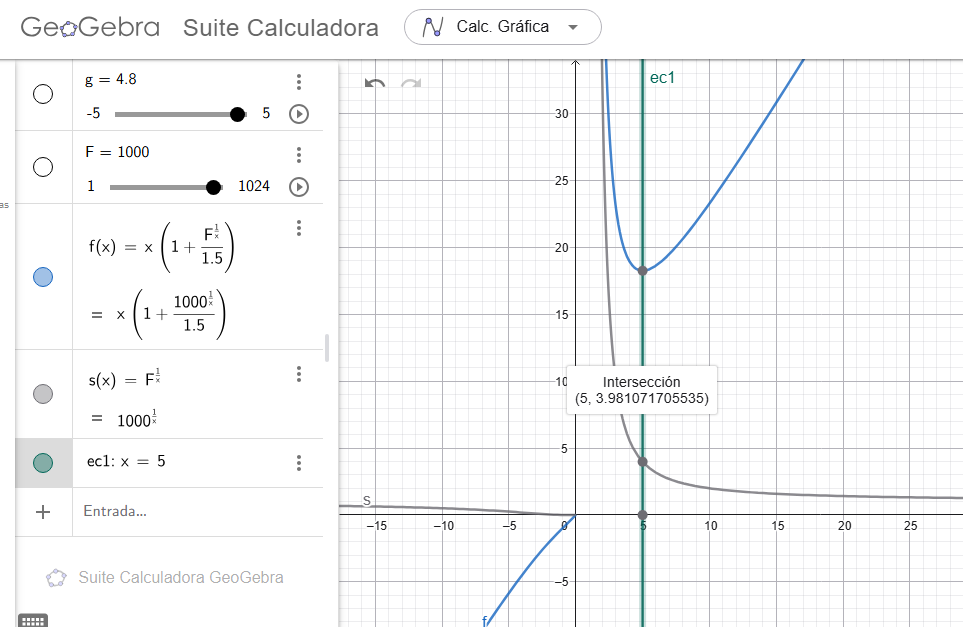
\includegraphics[width=0.6\textwidth]{./img/geogebra.png}
    \caption{Valor del fanout f optimo para un fanout total F=1000}
        \label{geogebra1}
\end{figure}
\begin{figure}[h]
    \centering
    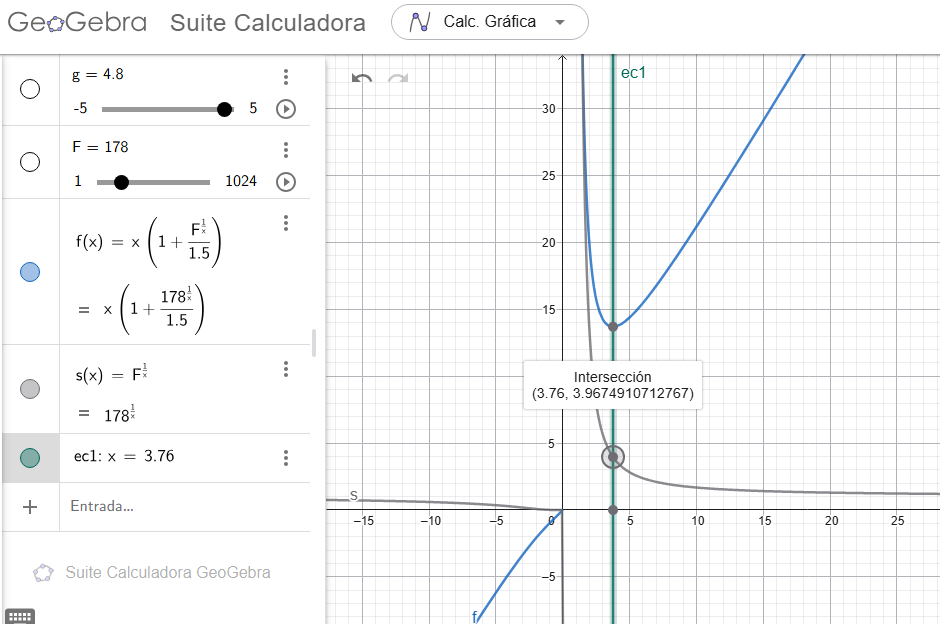
\includegraphics[width=0.6\textwidth]{./img/geogebra2.png}
    \caption{Valor del fanout f optimo para otro fanout total F=178}
        \label{geogebra2}
\end{figure}


Podemos entonces, encontrar el numero de etapas como 
$$N = ln(C_{load} / C_{in}) / ln(4)=log_4(C_{load}/C_{in}$$
---------------------------------------------

El sistema requiere varias cadenas de buffers para manejar las cargas capacitivas de los diferentes bloques. A continuación se indica como se encontaron las cargas capacitivas a manejar. Se consideró como inversor mínimo, un con $W_n = 0,15\mu m$  y $W_p = 0,3\mu m$ además $L_n=L_p=L_{min}=0,13\mu m$  por lo que para calcular la $C_{LOAD}$ se procedió de la siguiente manera, aproximando las capacitancias de compuerta  de ambos MOS al mismo valor, (suponemos esto debido a las similitudes de los valores reportados de CJUNCTION y CMILLER proporcionados por la documentación del proceso) \cite{IHP-sg13g2}:
\begin{itemize}
\item Multiplica $W$ por $m$ de cada transistor conectado al nodo, y luego se suma todo. 
\item Se divide el valor en 0,45 $\mu m$ para obtner la capacidad del nodo relativa a la capacidad de entrada de un inversor unitario 
\end{itemize}


\subsubsection{Buffer de Salidas del Comparador}

La salida del comparador maneja el latch que retiene la última comparación. Se implementó una cadena de buffers para:
\begin{itemize}
    \item Aislar el nodo de salida sensible del comparador, esto evita introducir offset y degradar demasiado el tiempo de conversión por el estado del latch. En el nodo de salida se conecta el inversor unitario
    \item Proveer drive suficiente para el latch.
\end{itemize}

En \cref{bufcompretardo} se muestran los retardos obtenidos. En este caso de 11ps desde que el comparador toma la decision (cuando una salida empieza a bajar) hasta el 50\% de VDD en la salida del buffer,.
\begin{figure}[H]
    \centering
    \includesvg[width=\linewidth]{retardo_buffer_comp}
    \caption{Retardo del buffer de la salida del comparador hacia el latch}
    \label{bufcompretardo}
\end{figure}

$$F_{LOAD} = 24$$

\subsubsection{Buffer de Salida Pulse del Comparador}
La salida que implementa el reloj del comparador mueve varios nodos
\begin{itemize}
    \item Señales di\_clk y di\_clk\_n del preamp y el latch
    \item Señal de reloj de la lógica
    \item di\_clk\_n y reloj logica $C_{LOAD} = 218 $
    \item di\_clk $C_{LOAD} = 48 $
\end{itemize}




% FIGURA: Cadena de buffers de salida del comparador con sizing

\subsubsection{Buffer de Señales de Lógica a CDAC}

Las señales de control digitales ($D[n]$ y $B[n]$) provenientes de la lógica SAR deben manejar todos los switches del CDAC. Se implementó una cadena de buffers para garantizar tiempos de rise/fall adecuados. Por cada transistor pmos unitario son 4.44  $C_{inv}$ y el nmos 2.22  $C_{inv}$ aproximadamente. tendremos entonces 3 buffers diferentes a implementar.
$$F_{TG_{nmos}} = n*2.22$$
$$F_{TG_{pmos}} = n*4.44$$
$$F_{nmos} = n*2.22$$
$$F_{pmos} = n*4.44$$


% FIGURA: Cadena de buffers para señales D y B con sizing



\subsubsection{Buffer de Señales de Sampleo}

Las señales non-overlap generadas deben manejar la carga capacitiva de todos los switches del array de muestreo. Para garantizar tiempos de rise/fall adecuados y evitar degradación de las señales, se implementó una cadena de buffers.De forma similar al caso anterior, pero esta vez con un numero fijo de transistores por nodo. Tenemos 2 dac (p y n) con 2 subdac, cada uno con 63 transistores, además tengamos en cuenta que la señal B maneja compuertas con dummmies asi que agregamos sus capaciades.
\begin{itemize}
    \item En el nodo Sample A se conectan 252 nmos
    \item En el nodo Sample B se conectan 378 pmos (por los dummmies)
    \item En el nodo Sample A negado se conectan 252 pmos
    \item En el nodo Sample B negado se conectan 378 nmos (por los dummmies)
\end{itemize}

$$F_{LOAD sample A} = 252*2.2=554.4$$
$$F_{LOAD sample B} = 378*4.4=1663$$
$$F_{LOAD sample A n} = 252*4.4=1108$$
$$F_{LOAD sample B n} = 378*2.2=831$$


\begin{table}[h]
\centering
\caption{Diseño de cadenas de buffers - Cálculo de etapas y multiplicadores}
\label{tab:buffer_chain_detailed}
\begin{tabular}{cccc}
\toprule
\textbf{$F_{LOAD}$} & \textbf{Número de etapas} & \textbf{Número de} & \textbf{Multiplicadores} \\
 & \textbf{(cálculo)} & \textbf{Etapas} & \\
\midrule
24 & 2.29248125 & 2 & 4-8 \\
48 & 2.79248125 & 2 & 4-8 \\
218 & 3.88409162 & 3 & 4-8-32 \\
554 & 4.56687083 & 4 & 4-8-32-64 \\
1663 & 5.34978627 & 5 & 4-8-32-64-256 \\
1108 & 5.05687083 & 5 & 4-8-32-64-256 \\
831 & 4.84935233 & 4 & 4-8-32-64 \\
4.44 & 1.07527983 & 1 & -- \\
8.88 & 1.57527983 & 1 & -- \\
17.76 & 2.07527983 & 2 & 4-8 \\
35.52 & 2.57527983 & 2 & 4-8 \\
71.04 & 3.07527983 & 3 & 4-8-32 \\
8.88 & 1.57527983 & 1 & -- \\
17.76 & 2.07527983 & 2 & 4-8 \\
35.52 & 2.57527983 & 2 & 4-8 \\
71.04 & 3.07527983 & 3 & 4-8-32 \\
142.08 & 3.57527983 & 3 & 4-8-32 \\
\bottomrule
\end{tabular}
\end{table}
\newpage
\section{Lógica SAR}
\begin{figure}[H]
    \centering
    \includesvg[width=\linewidth]{logica_parte}
    \caption{Fragmento de la cadena de la lógica implementada}
        \label{logfrag}
\end{figure}
La lógica SAR controla la secuencia de conversión y almacena los bits resueltos. Se implementó de manera síncrona utilizando celdas estándar del PDK ihp-sg13g2 formando una cadena "dominó" que activa la señal de decidido y retiene el bit a medida que recibe un 1 (desde D[n-1]) de la celda anterior, como se indica en \cref{logfrag} mostrando solo el principio de esta cadena que termina con la celda que maneja D[0] y B[0] .
Cada bloque unitario de la lógica consiste en 2 partes:
\begin{itemize}
\item El latch que guarda decidido, que propaga el valor logico alto en cada pulso generado por la decisión del comparador. Genera la señal D[n]

\item El latch que retiene el valor de la decisión del comparador de ese momento. Genera la señal Bit[n]
\end{itemize}


\subsection{Bloque Unitario de Lógica}

\begin{figure}[H]
    \centering
    \includesvg[width=\linewidth]{bit_cell_diagrama}
    \caption{Bloque unitario de la lógica, genera el bit B[n] y la señal de decidido D[n]}
        \label{logunitbit}
\end{figure}b
En \cref{logunitbit} se muestra el diagrama de cada eslabón que forma la cadena "dominó" de la logica.
La celda lógica sg13g2\_dfrbp\_1 implementa un flip-flop tipo D, activado por flanco con reset asincrónico activo bajo. La caracterizacion (tabla de verdad, delays) puede verse en:  \cite{IHP-sg13g2}\\

Cada bit de la conversión requiere un bloque de lógica que incluye:
\begin{itemize}
    \item Registro para retener el bit de decidido $D[n]$
    \item Biestable para retener el bit de control $B[n]$
    \item Lógica combinacional para generar señales de control del CDAC (En la implementación Layout)
    \item Interfaz con el bit anterior $D[n-1]$ para propagar la habilitación
\end{itemize}

\subsubsection{Entradas y Salidas del Bloque Unitario}

\textbf{Entradas:}
\begin{itemize}
    \item Salida del comparador (decisión del bit actual)
    \item Pulso del generador de pulsos (reloj de la lógica)
    \item $D[n-1]$ (habilitación desde el bit anterior)
\end{itemize}

\subsubsection{Entradas y Salidas del Bloque Unitario}

\textbf{Entradas:}
\begin{itemize}
    \item Salida del comparador (decisión del bit actual)
    \item Señal de Reset

\end{itemize}

\textbf{Salidas:}
\begin{itemize}
    \item $D[n]$: Señales de bits resueltos
    \item $B[n]$: Bit de control para el CDAC/Codigo de Salida 
\end{itemize}

% FIGURA: Diagrama de bloques del bloque unitario de lógica mostrando entradas, salidas y componentes internos

\subsection{Implementación con Celdas Estándar}

La implementación se realizó utilizando latches y compuertas lógicas de la biblioteca de celdas estándar del PDK ihp-sg13g2. Esto simplifica el diseño y garantiza:
\begin{itemize}
    \item Comportamiento lógico verificado
    \item Timing caracterizado
    \item Layout DRC-clean
\end{itemize}

% FIGURA: Esquemático del bloque unitario implementado con celdas estándar específicas


\subsection{Análisis de Timing}

\subsubsection{Delay de Propagación}

El parámetro crítico es el delay desde el flanco de subida del generador de pulsos hasta el cambio en las señales $D[n]$ y $B[n]$ que controlan el CDAC.

Este delay debe ser suficientemente pequeño para que:
\begin{equation}
T_{bit} = T_{reset} + T_{logic} + T_{comp} < T_{periodo}
\end{equation}

\subsubsection{Medición del Delay}

Se realizó simulación transitoria midiendo:
\begin{itemize}
    \item Delay de flanco de subida del generador de pulsos al cambio en $D[n]$
    \item Delay de flanco de subida del generador de pulsos al cambio en $B[n]$
    \item Variación del delay a lo largo de la cadena (bit 1 vs bit 12)
\end{itemize}
Se midió el delay desde el flanco de subida de clk hasta el flanco de subida  de las señales de la celda unitaria de lógica. Esto es porque ambas señales de salida siempre inician en 0. Se midió el delay en la simulación TOP, es decir con la lógica cargada.
% FIGURA: Forma de onda mostrando el pulso del generador y los cambios en D y B con marcadores de tiempo

\begin{table}[H]
\centering
\caption{Parámetros de Timing de la Lógica SAR}
    \label{logretardostab}
\begin{tabular}{|l|c|}
\hline
\textbf{Parámetro} & \textbf{Valor} \\
\hline
Delay pulso → $D[n]$ & $258$ ps \\
Delay pulso → $B[n]$ & $115$ ps \\

\hline
\end{tabular}
\end{table}


\section{Simulación TOP}
Se realizaron simulaciones tran a nivel TOP, usando entradas DC para probar la funcionalidad del circuito. Se muestra el testbench utilizado en \cref{toptb} mientras que las salidas obtenidas pueden verse en \cref{topssalidas} y el proceso de aproximaciones sucesivas en la salida del dac se ilustra en \cref{topsen}. Finalmente podemos ver como la entrada del comparador decrece monotonamente en \cref{convcomp}


\begin{figure}[H]
    \centering
    \includesvg[width=\linewidth]{conversion_ejemplo_1}
    \caption{Ejemplo de una conversión completa, se observa como el resultado se va a aproximando al valor de la entrada}
        \label{topsen}
\end{figure}

\begin{figure}[H]
    \centering
    \includesvg[width=\linewidth]{salidas_sar_ej1}
    \caption{Salidas correspondientes al ejemplo}
        \label{topssalidas}
\end{figure}

\begin{figure}[H]
    \centering
    \includesvg[width=\linewidth]{conversion_comparador_1}
    \caption{Entradas del comparador en el ejemplo (se escaló el clk para mejor visualizacion)}
        \label{convcomp}
\end{figure}

\subsection{Caracterización}
Se realizaron simulaciones con entrada DC para aproximar la longitud de los intervalos correspondientes a los códigos de $V_{in}=0$,$V_{in}=V_{DD}$ y $V_{in}=\frac{V_{DD}}{2}$, para lo cual se simularon 4 valores en los supuestos intervalos entre el codigo en cuestion y el anterior/siguiente. Se detalla los valores obtenidos en \cref{tab:adc_measurements}:
\begin{table}[H]
\centering
\caption{Resultados de simulación: Verificación de códigos y transiciones (Valores en mV).}
\label{tab:adc_measurements}
\renewcommand{\arraystretch}{1.2}
\begin{tabular}{@{}
  c
  S[table-format=4.3] % Formato para la columna LSB
  S[table-format=4.6] % Formato para la columna Vin
  c
  c
@{}}
\toprule
\textbf{Región} & {\textbf{Posición (LSB)}} & {\textbf{$V_{in}$ (mV)}} & \textbf{Cód. Esperado} & \textbf{Cód. Obtenido} \\ \midrule

% BLOQUE 0
\multirow{4}{*}{\shortstack{Código 0\\(Inicio)}} 
 & 0.125 & 0.109863 & 0 & \textbf{0} \\
 & 0.250 & 0.219726 & 0 & \textbf{0} \\
 & 0.375 & 0.329589 & 0 & \textbf{0} \\
 & 0.500 & 0.439453 & 0/1 (Transición) & \textbf{0} \\ \midrule

% BLOQUE 1024
\multirow{8}{*}{\shortstack{Código 1024\\(Mitad)}} 
 & 1023.500 & 899.560291 & 1023/1024 & \textbf{1023} \\
 & 1023.625 & 899.670154 & 1024 & \textbf{1024} \\
 & 1023.750 & 899.780017 & 1024 & \textbf{1024} \\
 & 1023.875 & 899.889880 & 1024 & \textbf{1024} \\
 & 1024.125 & 900.109607 & 1024 & \textbf{1024} \\
 & 1024.250 & 900.219470 & 1024 & \textbf{1024} \\
 & 1024.375 & 900.329333 & 1024 & \textbf{1024} \\
 & 1024.500 & 900.439197 & 1024/1025 & \textbf{1024} \\ \midrule

% BLOQUE 2048
\multirow{4}{*}{\shortstack{Código 2048\\(Final)}} 
 & 2047.500 & 1799.560035 & 2047/2048 & \textbf{2047} \\
 & 2047.625 & 1799.669898 & 2048 & \textbf{2048} \\
 & 2047.750 & 1799.779762 & 2048 & \textbf{2048} \\
 & 2047.875 & 1799.889625 & 2048 & \textbf{2048} \\ \bottomrule
\end{tabular}
\end{table}

\chapter{Diseño de Layout}
\section{Preamplificador}
\begin{figure}[H]
	\centering
	\includesvg[
	width=\linewidth,
	height=0.7\textheight,
	keepaspectratio
	]{img/lo_comp_preamp_scap}
	\caption{Layout del preamplificador, ocultando los capacitores}
	\label{preamp_lo}
\end{figure}

\begin{figure}[H]
	\centering
	\includesvg[
	width=\linewidth,
	height=0.7\textheight,
	keepaspectratio
	]{img/lo_comp_preamp_fl}
	\caption{Layout del preamplificador, mostrando todas las capas}
	\label{preamp_lo}
\end{figure}




\chapter{Conclusiones y Trabajo Futuro}

\section{Estado Actual del Trabajo}

Este documento presenta la implementación de un ADC SAR de 12 bits utilizando herramientas de código abierto y la tecnología ihp-sg13g2. Al momento de esta versión del informe, el diseño esquemático y las simulaciones funcionales están completos, y se ha avanzado significativamente en el layout físico. Se han completado y verificado (DRC/LVS) los siguientes bloques: comparador, celda unitaria del CDAC, latch del comparador, y generador de pulsos (implementado con transistores NMOS en triple-well). Sin embargo, el layout completo del sistema integrado y las simulaciones post-layout están pendientes para la versión final de este trabajo.

\section{Conclusiones}

\subsection{Logros Principales}

El presente trabajo ha logrado diseñar e implementar un ADC SAR de 12 bits funcional en tecnología ihp-sg13g2, cumpliendo con los objetivos establecidos:

\begin{itemize}
    \item \textbf{Diseño Funcional Completo:} Se implementó exitosamente un ADC SAR de 12 bits basado en la arquitectura IMCS (Inverted Merged Capacitor Switching), incluyendo todos los bloques necesarios: CDAC split-binary (6+6 bits), circuito de Sample \& Hold, comparador de doble cola tipo Bindra, generador de pulsos auto-sincronizado, y lógica SAR implementada con celdas estándar.
    
    \item \textbf{Rendimiento Alcanzado:} Las simulaciones funcionales demostraron que el diseño logra resolver conversiones dentro del error de cuantización esperado, con un tiempo de conversión promedio de aproximadamente 18 ns y un consumo energético de aproximadamente 220 pJ por conversión.
    
    \item \textbf{Verificación de Layout:} Los bloques de layout completados (comparador, celda unitaria del CDAC, latch del comparador, y generador de pulsos) pasaron exitosamente las verificaciones DRC (Design Rule Check) y LVS (Layout vs Schematic), demostrando la manufacturabilidad del diseño en el PDK ihp-sg13g2.
    
    \item \textbf{Documentación Completa:} Se logró el objetivo principal de proveer una guía didáctica exhaustiva del proceso de diseño de circuitos integrados analógicos utilizando exclusivamente herramientas de código abierto (xschem, ngspice, klayout). Todo el código, esquemáticos, scripts y resultados están disponibles públicamente en el repositorio~\cite{repo_SAR}.
    
    \item \textbf{Especificaciones como Baseline:} Aunque este diseño no fue optimizado exhaustivamente, las métricas obtenidas pueden servir como especificaciones mínimas para futuros diseños más sistemáticos. Las siguientes métricas fueron caracterizadas:
    \begin{itemize}
        \item Tiempo de conversión: $\sim$18 ns/conversión
        \item Energía por conversión: $\sim$220 pJ/conversión
        \item Figura de mérito (FoM): $\sim$ $14$ pJ/conversión-paso (estimado)
        \item Resolución funcional: 12 bits dentro del error de cuantización
    \end{itemize}
\end{itemize}

\subsection{Lecciones Aprendidas y Recomendaciones Metodológicas}

Durante el desarrollo de este trabajo se identificaron varios aspectos metodológicos que pueden ser de utilidad para futuros diseñadores:





\subsubsection{Simulaciones y Herramientas}

Los tiempos de simulación prolongados complicaron significativamente el análisis de performance. En ocasiones, el simulador presentaba problemas de convergencia que requerían ajustes en las condiciones iniciales o en el paso de integración. \textbf{Recomendación:} Un mejor entendimiento y práctica con ngspice acelera enormemente el trabajo. En particular, aprender a utilizar los comandos \texttt{.measure} para extracción automática de mediciones y el modo interactivo de ngspice fueron puntos de inflexión que mejoraron sustancialmente la productividad. 

El uso de foros especializados como FOSSI-chat resultó invaluable, permitiendo contacto directo con desarrolladores de las herramientas para resolver problemas específicos. \textbf{Recomendación:} Participar activamente en las comunidades de código abierto no solo acelera la resolución de problemas, sino que también contribuye al ecosistema general.

\subsubsection{Documentación Continua}

Un error metodológico importante fue dejar la documentación para las etapas finales del proyecto. Esto no solo dificultó recordar detalles específicos de las decisiones de diseño, sino que también privó al proceso de los beneficios de la escritura reflexiva. \textbf{Recomendación:} Escribir los resultados e ideas de manera continua es extremadamente útil para entender mejor lo que se está haciendo, identificar inconsistencias, y mantener un registro preciso de las decisiones de diseño y sus justificaciones.

\section{Trabajo Futuro}

\subsection{Mejoras en Metodología y Automatización}

\subsubsection{Automatización de Simulaciones}

Un punto de partida valioso para mejorar la eficiencia del flujo de diseño sería la automatización completa de las simulaciones, incluyendo:
\begin{itemize}
    \item Scripts para ejecutar baterías de simulaciones paramétricas
    \item Extracción automática de métricas utilizando comandos \texttt{.measure}
    \item Ordenamiento automático de resultados, gráficos e imágenes
    \item Generación automática de reportes con las métricas extraídas
\end{itemize}

Esta automatización permitiría explorar el espacio de diseño de manera mucho más eficiente y facilitaría el análisis de sensibilidad paramétrica.

\subsubsection{Diseño Basado en Corners}

Aunque no se puede modelar mismatch en simulaciones esquemáticas, sería extremadamente útil poder realizar simulaciones automáticas para diseñar sistemas que cumplan especificaciones en todos los corners de proceso, voltaje y temperatura (PVT). Esto permitiría garantizar robustez del diseño antes de proceder al layout.

\subsection{Mejoras Específicas del ADC}

\subsubsection{Implementación de Bootstrap Switches}

Una mejora significativa en la linealidad del ADC sería la implementación de switches bootstrapped según la técnica propuesta por Chang~\cite{chang_sar_thesis}. Estos switches deberían implementarse en:
\begin{itemize}
    \item Switches de muestreo (Sample \& Hold)
    \item Switches del CDAC que conectan a las entradas
    \item Potencialmente switches que conectan a $V_{CM}$
\end{itemize}

La implementación de bootstrap mejoraría la resistencia ON constante a lo largo del rango de entrada, reduciendo la distorsión armónica total (THD) y mejorando el SFDR del conversor.

\subsubsection{Comparación con Arquitectura de Top-Plate Sampling}

Sería valioso comparar el desempeño de la arquitectura IMCS implementada con una arquitectura MCS estándar que utiliza top-plate sampling. Esta comparación permitiría cuantificar experimentalmente los beneficios de la insensibilidad a parásitos de la IMCS versus la simplicidad del muestreo top-plate.

\subsection{Análisis Avanzados}

\subsubsection{Caracterización con Entradas Aleatorias}

Aunque no es posible simular mismatch directamente, se podrían realizar simulaciones con entradas aleatorias para obtener métricas que se ven degradadas por efectos dinámicos:
\begin{itemize}
    \item Offset dinámico del comparador
    \item Efectos de kickback sobre el CDAC
    \item Settling errors bajo diferentes condiciones de entrada
    \item Variación del tiempo de conversión con la amplitud de entrada
\end{itemize}

Este análisis proveería información valiosa sobre el comportamiento real del ADC en condiciones operativas variadas.

\subsubsection{Análisis de Parásitos por Bloque}

Un estudio sistemático de los efectos de parásitos individuales por bloque sería extremadamente útil para guiar el proceso de layout. Esto incluiría:
\begin{itemize}
    \item Degradación de la performance del comparador por parásitos en nodos críticos
    \item Impacto de resistencias serie en el CDAC sobre el settling time
    \item Efecto de capacitancias parásitas en el ancho de banda de buffers
    \item Sensibilidad del generador de pulsos a variaciones de parásitos
\end{itemize}

Este análisis permitiría priorizar esfuerzos de optimización de layout en los nodos más críticos.

\subsection{Mejoras de Layout}

\subsubsection{Layout con Common-Centroid}

Un buen punto de partida para mejorar el matching sería implementar el layout del comparador utilizando técnicas de common-centroid para los pares diferenciales. Esto reduciría el offset sistemático y mejoraría la simetría del diseño, sirviendo como ejemplo didáctico de técnicas avanzadas de layout.

El CDAC también se beneficiaría enormemente de un layout common-centroid para los arrays de capacitores, mejorando el matching entre capacitores unitarios y reduciendo errores de INL/DNL.

\subsubsection{Completar Layout del Sistema Integrado}

La finalización del layout completo y la realización de simulaciones post-layout con parásitos extraídos es el siguiente paso crítico. Esto permitirá:
\begin{itemize}
    \item Validar que el diseño mantiene funcionalidad con parásitos reales
    \item Cuantificar la degradación de performance por efectos de layout
    \item Identificar problemas de timing que no son visibles en simulaciones esquemáticas
    \item Completar la caracterización DNL/INL del sistema
\end{itemize}

\subsection{Escalabilidad: Arquitectura Time-Interleaved}

Un objetivo de largo plazo para este diseño es su uso como canal individual en una arquitectura time-interleaved. Este trabajo fue concebido como el primer paso hacia un ADC multi-canal de alta velocidad.

\subsubsection{Motivación}

La arquitectura time-interleaved permite escalar la velocidad de muestreo efectiva multiplicando el número de canales. Si este diseño alcanza 1 MSa/s por canal, un sistema de $N$ canales intercalados podría alcanzar $N$ MSa/s, extendiendo significativamente el rango de aplicaciones.

\subsubsection{Desafíos}

La implementación time-interleaved introduce nuevos desafíos:
\begin{itemize}
    \item \textbf{Offset mismatch:} Diferencias de offset entre canales generan espurios en el espectro de salida
    \item \textbf{Gain mismatch:} Diferencias de ganancia entre canales degradan SFDR
    \item \textbf{Timing skew:} Errores en el timing de muestreo entre canales limitan el SNDR a altas frecuencias de entrada
    \item \textbf{Complejidad de calibración:} Se requieren algoritmos de calibración digital para corregir mismatches
\end{itemize}

\subsubsection{Trabajo Futuro}

Una vez completado y caracterizado este diseño de canal único, el trabajo futuro incluiría:
\begin{enumerate}
    \item Optimización del canal único para minimizar área y consumo (facilitando la replicación)
    \item Diseño del sistema de generación de fases de reloj con bajo skew
    \item Implementación de múltiples canales con layout matched
    \item Desarrollo de algoritmos de calibración digital para corrección de offset, ganancia y timing
    \item Caracterización completa del sistema time-interleaved (SNDR vs frecuencia de entrada, SFDR, espurios por mismatch)
\end{enumerate}

Este trabajo sienta las bases para ese desarrollo futuro, proveyendo un diseño funcional, documentado y verificado que puede servir como punto de partida.

\section{Reflexión Final}

Este proyecto demuestra que es posible diseñar circuitos integrados analógicos complejos utilizando exclusivamente herramientas de código abierto y PDKs accesibles. Si bien el camino presentó desafíos metodológicos y técnicos, el resultado es un diseño funcional documentado que puede servir como material educativo y punto de partida para desarrollos futuros.

La disponibilidad completa del código, esquemáticos, scripts y documentación en el repositorio público contribuye al ecosistema de diseño de código abierto y facilita que otros estudiantes e investigadores puedan replicar, mejorar y extender este trabajo.

\begin{thebibliography}{99}

\bibitem{repo_SAR}
J. G. D. Avila, ``SAR ADC IHP Repository,'' GitHub, 2025. [Online]. Disponible: \url{https://github.com/gsuckz/SAR_ADC_IHP}

\bibitem{lowpower_survey} X. Tang et al., ``Low-Power SAR ADC Design: Overview and Survey of State-of-the-Art Techniques,'' \textit{IEEE TRANSACTIONS ON CIRCUITS AND SYSTEMS—I: REGULAR PAPERS, VOL. 69, NO. 6, JUNE 2022}.

\bibitem{murmann_sar} V. Tripathi and B. Murmann, "An 8-bit 450-MS/s single-bit/cycle SAR ADC in 65-nm CMOS," 2013 Proceedings of the ESSCIRC (ESSCIRC), Bucharest, Romania, 2013, pp. 117-120, doi: 10.1109/ESSCIRC.2013.6649086.

\bibitem{vanelzakker_sar} M. van Elzakker et al., ``A 10-bit charge-redistribution ADC consuming 1.9 $\mu W$ at 1 MS/s,'' \textit{IEEE J. Solid-State Circuits}, vol. 45, no. 5, pp. 1007–1015, May 2010.

\bibitem{bindra_comparator} H. S. Bindra et al., ``A 1.2-V dynamic bias latch-type comparator in 65-nm CMOS with 0.4-mV input noise,'' \textit{IEEE J. Solid-State Circuits}, vol. 53, no. 7, pp. 1902–1912, Jul. 2018.

\bibitem{iizuka_systematic} T. Iizuka, R. Takenaka, H. Xu and A. A. Abidi, "Systematic Equation-Based Design of a 10-Bit, 500-MS/s Single-Channel SAR A/D Converter With 2-GHz Resolution Bandwidth," in IEEE Open Journal of the Solid-State Circuits Society, vol. 4, pp. 147-162, 2024, doi: 10.1109/OJSSCS.2024.3469109

\bibitem{chang_sar_thesis} A. H. T. Chang, ``Low-Power High-Performance SAR ADC with Redundancy and Digital Background Calibration,'' Master's thesis, Massachusetts Institute of Technology, 2013.

\bibitem{IHP-sg13g2}
IHP GmbH, ``SG13G2 Open Source Layout Rules,'' \textit{IHP-Open-PDK GitHub Repository}. [Online]. Disponible: \url{https://github.com/IHP-GmbH/IHP-Open-PDK/blob/main/ihp-sg13g2/libs.doc/doc/SG13G2_os_layout_rules.pdf}

	
\bibitem{dorrer} An open-source adaptive event-based ADC for bio-signal acquisition in 130nm CMOS
Dorrer, Simon [VerfasserIn]; 2025

\bibitem{bwsah}
The Relationship Between Rise Time and Bandwidth in Digital Signals \textit{All About Circuits}. [Online]. Disponible: \url{https://www.allaboutcircuits.com/technical-articles/relationship-between-rise-time-bandwidth-digital-signal}

\bibitem{rabaey}
J. M. Rabaey, A. P. Chandrakasan y B. Nikolić, \textit{Digital Integrated Circuits: A Design Perspective}, 2.ª ed. Upper Saddle River, NJ: Prentice Hall, 2003.

\end{thebibliography}

% TODO: Agregar referencias adicionales


\end{document}